\documentclass[twoside]{book}

% Packages required by doxygen
\usepackage{calc}
\usepackage{doxygen}
\usepackage{graphicx}
\usepackage[utf8]{inputenc}
\usepackage{makeidx}
\usepackage{multicol}
\usepackage{multirow}
\usepackage{fixltx2e}
\PassOptionsToPackage{warn}{textcomp}
\usepackage{textcomp}
\usepackage[nointegrals]{wasysym}
\usepackage[table]{xcolor}

% Font selection
\usepackage[T1]{fontenc}
\usepackage{mathptmx}
\usepackage[scaled=.90]{helvet}
\usepackage{courier}
\usepackage{amssymb}
\usepackage{sectsty}
\renewcommand{\familydefault}{\sfdefault}
\allsectionsfont{%
  \fontseries{bc}\selectfont%
  \color{darkgray}%
}
\renewcommand{\DoxyLabelFont}{%
  \fontseries{bc}\selectfont%
  \color{darkgray}%
}
\newcommand{\+}{\discretionary{\mbox{\scriptsize$\hookleftarrow$}}{}{}}

% Page & text layout
\usepackage{geometry}
\geometry{%
  a4paper,%
  top=2.5cm,%
  bottom=2.5cm,%
  left=2.5cm,%
  right=2.5cm%
}
\tolerance=750
\hfuzz=15pt
\hbadness=750
\setlength{\emergencystretch}{15pt}
\setlength{\parindent}{0cm}
\setlength{\parskip}{0.2cm}
\makeatletter
\renewcommand{\paragraph}{%
  \@startsection{paragraph}{4}{0ex}{-1.0ex}{1.0ex}{%
    \normalfont\normalsize\bfseries\SS@parafont%
  }%
}
\renewcommand{\subparagraph}{%
  \@startsection{subparagraph}{5}{0ex}{-1.0ex}{1.0ex}{%
    \normalfont\normalsize\bfseries\SS@subparafont%
  }%
}
\makeatother

% Headers & footers
\usepackage{fancyhdr}
\pagestyle{fancyplain}
\fancyhead[LE]{\fancyplain{}{\bfseries\thepage}}
\fancyhead[CE]{\fancyplain{}{}}
\fancyhead[RE]{\fancyplain{}{\bfseries\leftmark}}
\fancyhead[LO]{\fancyplain{}{\bfseries\rightmark}}
\fancyhead[CO]{\fancyplain{}{}}
\fancyhead[RO]{\fancyplain{}{\bfseries\thepage}}
\fancyfoot[LE]{\fancyplain{}{}}
\fancyfoot[CE]{\fancyplain{}{}}
\fancyfoot[RE]{\fancyplain{}{\bfseries\scriptsize Generated on Tue Jun 24 2014 14\+:39\+:48 for G\+R-\/\+Router by Doxygen }}
\fancyfoot[LO]{\fancyplain{}{\bfseries\scriptsize Generated on Tue Jun 24 2014 14\+:39\+:48 for G\+R-\/\+Router by Doxygen }}
\fancyfoot[CO]{\fancyplain{}{}}
\fancyfoot[RO]{\fancyplain{}{}}
\renewcommand{\footrulewidth}{0.4pt}
\renewcommand{\chaptermark}[1]{%
  \markboth{#1}{}%
}
\renewcommand{\sectionmark}[1]{%
  \markright{\thesection\ #1}%
}

% Indices & bibliography
\usepackage{natbib}
\usepackage[titles]{tocloft}
\setcounter{tocdepth}{3}
\setcounter{secnumdepth}{5}
\makeindex

% Hyperlinks (required, but should be loaded last)
\usepackage{ifpdf}
\ifpdf
  \usepackage[pdftex,pagebackref=true]{hyperref}
\else
  \usepackage[ps2pdf,pagebackref=true]{hyperref}
\fi
\hypersetup{%
  colorlinks=true,%
  linkcolor=blue,%
  citecolor=blue,%
  unicode%
}

% Custom commands
\newcommand{\clearemptydoublepage}{%
  \newpage{\pagestyle{empty}\cleardoublepage}%
}


%===== C O N T E N T S =====

\begin{document}

% Titlepage & ToC
\hypersetup{pageanchor=false,
             bookmarks=true,
             bookmarksnumbered=true,
             pdfencoding=unicode
            }
\pagenumbering{roman}
\begin{titlepage}
\vspace*{7cm}
\begin{center}%
{\Large G\+R-\/\+Router \\[1ex]\large 1 }\\
\vspace*{1cm}
{\large Generated by Doxygen 1.8.7}\\
\vspace*{0.5cm}
{\small Tue Jun 24 2014 14:39:48}\\
\end{center}
\end{titlepage}
\clearemptydoublepage
\tableofcontents
\clearemptydoublepage
\pagenumbering{arabic}
\hypersetup{pageanchor=true}

%--- Begin generated contents ---
\chapter{Hierarchical Index}
\section{Class Hierarchy}
This inheritance list is sorted roughly, but not completely, alphabetically\+:\begin{DoxyCompactList}
\item child\begin{DoxyCompactList}
\item \contentsline{section}{gr\+:\+:router\+:\+:child\+\_\+impl}{\pageref{classgr_1_1router_1_1child__impl}}{}
\end{DoxyCompactList}
\item \contentsline{section}{Ethernet\+Connector}{\pageref{class_ethernet_connector}}{}
\item \contentsline{section}{Network\+Interface}{\pageref{class_network_interface}}{}
\item \contentsline{section}{Node}{\pageref{class_node}}{}
\item \contentsline{section}{qa\+\_\+router}{\pageref{classqa__router}}{}
\item queue\+\_\+sink\begin{DoxyCompactList}
\item \contentsline{section}{gr\+:\+:router\+:\+:queue\+\_\+sink\+\_\+impl}{\pageref{classgr_1_1router_1_1queue__sink__impl}}{}
\end{DoxyCompactList}
\item queue\+\_\+sink\+\_\+byte\begin{DoxyCompactList}
\item \contentsline{section}{gr\+:\+:router\+:\+:queue\+\_\+sink\+\_\+byte\+\_\+impl}{\pageref{classgr_1_1router_1_1queue__sink__byte__impl}}{}
\end{DoxyCompactList}
\item queue\+\_\+source\begin{DoxyCompactList}
\item \contentsline{section}{gr\+:\+:router\+:\+:queue\+\_\+source\+\_\+impl}{\pageref{classgr_1_1router_1_1queue__source__impl}}{}
\end{DoxyCompactList}
\item queue\+\_\+source\+\_\+byte\begin{DoxyCompactList}
\item \contentsline{section}{gr\+:\+:router\+:\+:queue\+\_\+source\+\_\+byte\+\_\+impl}{\pageref{classgr_1_1router_1_1queue__source__byte__impl}}{}
\end{DoxyCompactList}
\item root\begin{DoxyCompactList}
\item \contentsline{section}{gr\+:\+:router\+:\+:root\+\_\+impl}{\pageref{classgr_1_1router_1_1root__impl}}{}
\end{DoxyCompactList}
\item throughput\begin{DoxyCompactList}
\item \contentsline{section}{gr\+:\+:router\+:\+:throughput\+\_\+impl}{\pageref{classgr_1_1router_1_1throughput__impl}}{}
\end{DoxyCompactList}
\item throughput\+\_\+sink\begin{DoxyCompactList}
\item \contentsline{section}{gr\+:\+:router\+:\+:throughput\+\_\+sink\+\_\+impl}{\pageref{classgr_1_1router_1_1throughput__sink__impl}}{}
\end{DoxyCompactList}
\end{DoxyCompactList}

\chapter{Class Index}
\section{Class List}
Here are the classes, structs, unions and interfaces with brief descriptions\+:\begin{DoxyCompactList}
\item\contentsline{section}{\hyperlink{classgr_1_1router_1_1child__impl}{gr\+::router\+::child\+\_\+impl} }{\pageref{classgr_1_1router_1_1child__impl}}{}
\item\contentsline{section}{\hyperlink{class_ethernet_connector}{Ethernet\+Connector} }{\pageref{class_ethernet_connector}}{}
\item\contentsline{section}{\hyperlink{class_network_interface}{Network\+Interface} }{\pageref{class_network_interface}}{}
\item\contentsline{section}{\hyperlink{class_node}{Node} }{\pageref{class_node}}{}
\item\contentsline{section}{\hyperlink{classqa__router}{qa\+\_\+router} \\*Collect all the tests for the gr-\/filter directory }{\pageref{classqa__router}}{}
\item\contentsline{section}{\hyperlink{classgr_1_1router_1_1queue__sink__byte__impl}{gr\+::router\+::queue\+\_\+sink\+\_\+byte\+\_\+impl} }{\pageref{classgr_1_1router_1_1queue__sink__byte__impl}}{}
\item\contentsline{section}{\hyperlink{classgr_1_1router_1_1queue__sink__impl}{gr\+::router\+::queue\+\_\+sink\+\_\+impl} }{\pageref{classgr_1_1router_1_1queue__sink__impl}}{}
\item\contentsline{section}{\hyperlink{classgr_1_1router_1_1queue__source__byte__impl}{gr\+::router\+::queue\+\_\+source\+\_\+byte\+\_\+impl} }{\pageref{classgr_1_1router_1_1queue__source__byte__impl}}{}
\item\contentsline{section}{\hyperlink{classgr_1_1router_1_1queue__source__impl}{gr\+::router\+::queue\+\_\+source\+\_\+impl} }{\pageref{classgr_1_1router_1_1queue__source__impl}}{}
\item\contentsline{section}{\hyperlink{classgr_1_1router_1_1root__impl}{gr\+::router\+::root\+\_\+impl} }{\pageref{classgr_1_1router_1_1root__impl}}{}
\item\contentsline{section}{\hyperlink{classgr_1_1router_1_1throughput__impl}{gr\+::router\+::throughput\+\_\+impl} }{\pageref{classgr_1_1router_1_1throughput__impl}}{}
\item\contentsline{section}{\hyperlink{classgr_1_1router_1_1throughput__sink__impl}{gr\+::router\+::throughput\+\_\+sink\+\_\+impl} }{\pageref{classgr_1_1router_1_1throughput__sink__impl}}{}
\end{DoxyCompactList}

\chapter{Class Documentation}
\hypertarget{classgr_1_1router_1_1child__impl}{\section{gr\+:\+:router\+:\+:child\+\_\+impl Class Reference}
\label{classgr_1_1router_1_1child__impl}\index{gr\+::router\+::child\+\_\+impl@{gr\+::router\+::child\+\_\+impl}}
}
Inheritance diagram for gr\+:\+:router\+:\+:child\+\_\+impl\+:\begin{figure}[H]
\begin{center}
\leavevmode
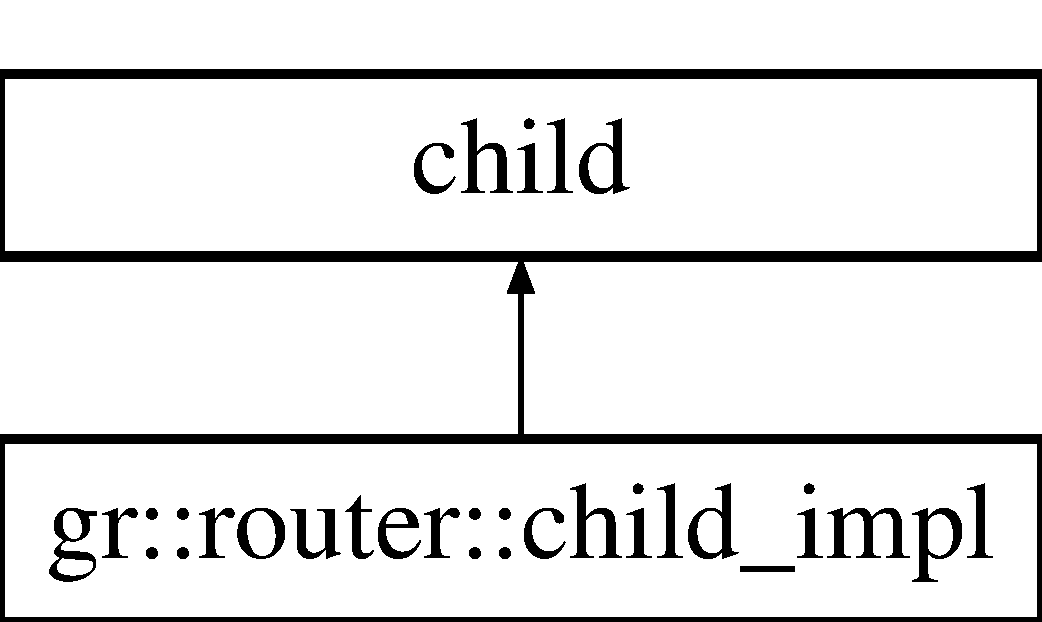
\includegraphics[height=2.000000cm]{classgr_1_1router_1_1child__impl}
\end{center}
\end{figure}
\subsection*{Public Member Functions}
\begin{DoxyCompactItemize}
\item 
\hyperlink{classgr_1_1router_1_1child__impl_aabaff6e60fad3c91138087379a7aa5d3}{child\+\_\+impl} (int number\+\_\+of\+\_\+children, int child\+\_\+index, char $\ast$hostname, boost\+::lockfree\+::queue$<$ std\+::vector$<$ float $>$ $\ast$, boost\+::lockfree\+::fixed\+\_\+sized$<$ true $>$ $>$ \&in\+\_\+queue, boost\+::lockfree\+::queue$<$ std\+::vector$<$ char $>$ $\ast$, boost\+::lockfree\+::fixed\+\_\+sized$<$ true $>$ $>$ \&out\+\_\+queue, double throughput)
\item 
\hyperlink{classgr_1_1router_1_1child__impl_a65c85e62fd693c4a87811f73c7e6234b}{$\sim$child\+\_\+impl} ()
\item 
int \hyperlink{classgr_1_1router_1_1child__impl_a7a429a34494106bd743e5515eacc6605}{work} (int noutput\+\_\+items, gr\+\_\+vector\+\_\+const\+\_\+void\+\_\+star \&input\+\_\+items, gr\+\_\+vector\+\_\+void\+\_\+star \&output\+\_\+items)
\end{DoxyCompactItemize}


\subsection{Constructor \& Destructor Documentation}
\hypertarget{classgr_1_1router_1_1child__impl_aabaff6e60fad3c91138087379a7aa5d3}{\index{gr\+::router\+::child\+\_\+impl@{gr\+::router\+::child\+\_\+impl}!child\+\_\+impl@{child\+\_\+impl}}
\index{child\+\_\+impl@{child\+\_\+impl}!gr\+::router\+::child\+\_\+impl@{gr\+::router\+::child\+\_\+impl}}
\subsubsection[{child\+\_\+impl}]{\setlength{\rightskip}{0pt plus 5cm}gr\+::router\+::child\+\_\+impl\+::child\+\_\+impl (
\begin{DoxyParamCaption}
\item[{int}]{numberofchildren, }
\item[{int}]{index, }
\item[{char $\ast$}]{hostname, }
\item[{boost\+::lockfree\+::queue$<$ std\+::vector$<$ float $>$ $\ast$, boost\+::lockfree\+::fixed\+\_\+sized$<$ true $>$ $>$ \&}]{input\+\_\+queue, }
\item[{boost\+::lockfree\+::queue$<$ std\+::vector$<$ char $>$ $\ast$, boost\+::lockfree\+::fixed\+\_\+sized$<$ true $>$ $>$ \&}]{output\+\_\+queue, }
\item[{double}]{throughput}
\end{DoxyParamCaption}
)}}\label{classgr_1_1router_1_1child__impl_aabaff6e60fad3c91138087379a7aa5d3}
This is the private constructor for the child router block.


\begin{DoxyParams}{Parameters}
{\em number\+\_\+of\+\_\+children} & The number of children that the child router has. (0 for now) \\
\hline
{\em child\+\_\+index} & The index of this child. \\
\hline
{\em hostname} & The hostname (or ip address) of the child's parent. \\
\hline
{\em \&input\+\_\+queue} & A pointer to the input lockfree queue, where segments sent from the parent will be pushed. \\
\hline
{\em \&output\+\_\+queue} & A pointer to the output lockfree queue, where completed segments will be pulled from to send to the parent. \\
\hline
{\em throughput} & The maximum rate at which the child router will pull from the output queue. (Not currently being used) \\
\hline
\end{DoxyParams}
\hypertarget{classgr_1_1router_1_1child__impl_a65c85e62fd693c4a87811f73c7e6234b}{\index{gr\+::router\+::child\+\_\+impl@{gr\+::router\+::child\+\_\+impl}!````~child\+\_\+impl@{$\sim$child\+\_\+impl}}
\index{````~child\+\_\+impl@{$\sim$child\+\_\+impl}!gr\+::router\+::child\+\_\+impl@{gr\+::router\+::child\+\_\+impl}}
\subsubsection[{$\sim$child\+\_\+impl}]{\setlength{\rightskip}{0pt plus 5cm}gr\+::router\+::child\+\_\+impl\+::$\sim$child\+\_\+impl (
\begin{DoxyParamCaption}
{}
\end{DoxyParamCaption}
)}}\label{classgr_1_1router_1_1child__impl_a65c85e62fd693c4a87811f73c7e6234b}
The destructor for the child router block.

Interrupt and join all threads, and delete the Connector. 

\subsection{Member Function Documentation}
\hypertarget{classgr_1_1router_1_1child__impl_a7a429a34494106bd743e5515eacc6605}{\index{gr\+::router\+::child\+\_\+impl@{gr\+::router\+::child\+\_\+impl}!work@{work}}
\index{work@{work}!gr\+::router\+::child\+\_\+impl@{gr\+::router\+::child\+\_\+impl}}
\subsubsection[{work}]{\setlength{\rightskip}{0pt plus 5cm}int gr\+::router\+::child\+\_\+impl\+::work (
\begin{DoxyParamCaption}
\item[{int}]{noutput\+\_\+items, }
\item[{gr\+\_\+vector\+\_\+const\+\_\+void\+\_\+star \&}]{input\+\_\+items, }
\item[{gr\+\_\+vector\+\_\+void\+\_\+star \&}]{output\+\_\+items}
\end{DoxyParamCaption}
)}}\label{classgr_1_1router_1_1child__impl_a7a429a34494106bd743e5515eacc6605}
This is the \hyperlink{classgr_1_1router_1_1child__impl_a7a429a34494106bd743e5515eacc6605}{work()} function. It doesn't do anything, because all sending and receiving is done with separate threads. 

The documentation for this class was generated from the following files\+:\begin{DoxyCompactItemize}
\item 
lib/child\+\_\+impl.\+h\item 
lib/child\+\_\+impl.\+cc\end{DoxyCompactItemize}

\hypertarget{class_ethernet_connector}{\section{Ethernet\+Connector Class Reference}
\label{class_ethernet_connector}\index{Ethernet\+Connector@{Ethernet\+Connector}}
}
\subsection*{Public Member Functions}
\begin{DoxyCompactItemize}
\item 
\hyperlink{class_ethernet_connector_ad9c57f606bb89e55c8b2b9a368ddb7d7}{Ethernet\+Connector} (int number\+\_\+of\+\_\+children, int port)
\item 
\hyperlink{class_ethernet_connector_a0e4bbc154a90b5215c677fc8934ddc41}{$\sim$\+Ethernet\+Connector} ()
\item 
bool \hyperlink{class_ethernet_connector_ac87a2cd96046fbf4576c3be120a38bdc}{connect\+\_\+to\+\_\+parent} (char $\ast$hostname, int port)
\item 
int \hyperlink{class_ethernet_connector_a5e3daf8069bf7fdc1ebc96d33c03dd62}{write\+\_\+parent} (char $\ast$msg, int size)
\item 
int \hyperlink{class_ethernet_connector_a7594171ffb3c6f4de4bdf32f9b9b56cc}{read\+\_\+parent} (char $\ast$outbuf, int size)
\item 
bool \hyperlink{class_ethernet_connector_a2cb599573bc7db2e92a9c22d302f58ea}{connect\+\_\+to\+\_\+child} (int index, int port)
\item 
int \hyperlink{class_ethernet_connector_a44b4142c65e12b9dba201a840b09a02b}{write\+\_\+child} (int index, char $\ast$inbuf, unsigned long size)
\item 
int \hyperlink{class_ethernet_connector_a5589ca816791a3b2dbce8a50e401b72e}{read\+\_\+child} (int index, char $\ast$outbuf, int size)
\item 
void \hyperlink{class_ethernet_connector_a76621c514770ab7702cf9881c719715c}{stop} ()
\end{DoxyCompactItemize}


\subsection{Constructor \& Destructor Documentation}
\hypertarget{class_ethernet_connector_ad9c57f606bb89e55c8b2b9a368ddb7d7}{\index{Ethernet\+Connector@{Ethernet\+Connector}!Ethernet\+Connector@{Ethernet\+Connector}}
\index{Ethernet\+Connector@{Ethernet\+Connector}!Ethernet\+Connector@{Ethernet\+Connector}}
\subsubsection[{Ethernet\+Connector}]{\setlength{\rightskip}{0pt plus 5cm}Ethernet\+Connector\+::\+Ethernet\+Connector (
\begin{DoxyParamCaption}
\item[{int}]{count, }
\item[{int}]{port}
\end{DoxyParamCaption}
)}}\label{class_ethernet_connector_ad9c57f606bb89e55c8b2b9a368ddb7d7}
This is the public constuctor for the Ethernet Connector.


\begin{DoxyParams}{Parameters}
{\em count} & The number of children that the router will connect to. \\
\hline
{\em port} & The port on which the router will communicate. \\
\hline
\end{DoxyParams}
\hypertarget{class_ethernet_connector_a0e4bbc154a90b5215c677fc8934ddc41}{\index{Ethernet\+Connector@{Ethernet\+Connector}!````~Ethernet\+Connector@{$\sim$\+Ethernet\+Connector}}
\index{````~Ethernet\+Connector@{$\sim$\+Ethernet\+Connector}!Ethernet\+Connector@{Ethernet\+Connector}}
\subsubsection[{$\sim$\+Ethernet\+Connector}]{\setlength{\rightskip}{0pt plus 5cm}Ethernet\+Connector\+::$\sim$\+Ethernet\+Connector (
\begin{DoxyParamCaption}
{}
\end{DoxyParamCaption}
)}}\label{class_ethernet_connector_a0e4bbc154a90b5215c677fc8934ddc41}
This is the destructor for the Ethernet Connector. 

\subsection{Member Function Documentation}
\hypertarget{class_ethernet_connector_a2cb599573bc7db2e92a9c22d302f58ea}{\index{Ethernet\+Connector@{Ethernet\+Connector}!connect\+\_\+to\+\_\+child@{connect\+\_\+to\+\_\+child}}
\index{connect\+\_\+to\+\_\+child@{connect\+\_\+to\+\_\+child}!Ethernet\+Connector@{Ethernet\+Connector}}
\subsubsection[{connect\+\_\+to\+\_\+child}]{\setlength{\rightskip}{0pt plus 5cm}bool Ethernet\+Connector\+::connect\+\_\+to\+\_\+child (
\begin{DoxyParamCaption}
\item[{int}]{index, }
\item[{int}]{port}
\end{DoxyParamCaption}
)}}\label{class_ethernet_connector_a2cb599573bc7db2e92a9c22d302f58ea}
This function will connect the router to it's child


\begin{DoxyParams}{Parameters}
{\em index} & The index of the child to connect to. \\
\hline
{\em port} & The port on which the router will communicate with its child on. \\
\hline
\end{DoxyParams}
\hypertarget{class_ethernet_connector_ac87a2cd96046fbf4576c3be120a38bdc}{\index{Ethernet\+Connector@{Ethernet\+Connector}!connect\+\_\+to\+\_\+parent@{connect\+\_\+to\+\_\+parent}}
\index{connect\+\_\+to\+\_\+parent@{connect\+\_\+to\+\_\+parent}!Ethernet\+Connector@{Ethernet\+Connector}}
\subsubsection[{connect\+\_\+to\+\_\+parent}]{\setlength{\rightskip}{0pt plus 5cm}bool Ethernet\+Connector\+::connect\+\_\+to\+\_\+parent (
\begin{DoxyParamCaption}
\item[{char $\ast$}]{hostname, }
\item[{int}]{port}
\end{DoxyParamCaption}
)}}\label{class_ethernet_connector_ac87a2cd96046fbf4576c3be120a38bdc}
Connect to the parent.


\begin{DoxyParams}{Parameters}
{\em hostname} & The hostname / ip address of the parent node to connect to. \\
\hline
{\em port} & The port for the child to connect to the parent on. \\
\hline
\end{DoxyParams}
\begin{DoxyReturn}{Returns}
bool Return True if the node could connect to it's parent; False if not. 
\end{DoxyReturn}
\hypertarget{class_ethernet_connector_a5589ca816791a3b2dbce8a50e401b72e}{\index{Ethernet\+Connector@{Ethernet\+Connector}!read\+\_\+child@{read\+\_\+child}}
\index{read\+\_\+child@{read\+\_\+child}!Ethernet\+Connector@{Ethernet\+Connector}}
\subsubsection[{read\+\_\+child}]{\setlength{\rightskip}{0pt plus 5cm}int Ethernet\+Connector\+::read\+\_\+child (
\begin{DoxyParamCaption}
\item[{int}]{index, }
\item[{char $\ast$}]{outbuf, }
\item[{int}]{size}
\end{DoxyParamCaption}
)}}\label{class_ethernet_connector_a5589ca816791a3b2dbce8a50e401b72e}
Read from the child at index Children\mbox{[}index\mbox{]}


\begin{DoxyParams}{Parameters}
{\em index} & The index of the child to read from. \\
\hline
{\em outbuf} & A pointer to an array of characters to write the data into. \\
\hline
\end{DoxyParams}
\begin{DoxyReturn}{Returns}
r The number of bytes read from the child. 
\end{DoxyReturn}
\hypertarget{class_ethernet_connector_a7594171ffb3c6f4de4bdf32f9b9b56cc}{\index{Ethernet\+Connector@{Ethernet\+Connector}!read\+\_\+parent@{read\+\_\+parent}}
\index{read\+\_\+parent@{read\+\_\+parent}!Ethernet\+Connector@{Ethernet\+Connector}}
\subsubsection[{read\+\_\+parent}]{\setlength{\rightskip}{0pt plus 5cm}int Ethernet\+Connector\+::read\+\_\+parent (
\begin{DoxyParamCaption}
\item[{char $\ast$}]{outbuf, }
\item[{int}]{size}
\end{DoxyParamCaption}
)}}\label{class_ethernet_connector_a7594171ffb3c6f4de4bdf32f9b9b56cc}
Read data from the parent.


\begin{DoxyParams}{Parameters}
{\em outbuf} & A pointer to a byte array where the data from the parent would be written to. \\
\hline
{\em size} & The number of bytes to be received from the parent. \\
\hline
\end{DoxyParams}
\begin{DoxyReturn}{Returns}
r The number of bytes received. 
\end{DoxyReturn}
\hypertarget{class_ethernet_connector_a76621c514770ab7702cf9881c719715c}{\index{Ethernet\+Connector@{Ethernet\+Connector}!stop@{stop}}
\index{stop@{stop}!Ethernet\+Connector@{Ethernet\+Connector}}
\subsubsection[{stop}]{\setlength{\rightskip}{0pt plus 5cm}void Ethernet\+Connector\+::stop (
\begin{DoxyParamCaption}
{}
\end{DoxyParamCaption}
)}}\label{class_ethernet_connector_a76621c514770ab7702cf9881c719715c}
Close the file descriptors between this node and its parent and children. \hypertarget{class_ethernet_connector_a44b4142c65e12b9dba201a840b09a02b}{\index{Ethernet\+Connector@{Ethernet\+Connector}!write\+\_\+child@{write\+\_\+child}}
\index{write\+\_\+child@{write\+\_\+child}!Ethernet\+Connector@{Ethernet\+Connector}}
\subsubsection[{write\+\_\+child}]{\setlength{\rightskip}{0pt plus 5cm}int Ethernet\+Connector\+::write\+\_\+child (
\begin{DoxyParamCaption}
\item[{int}]{index, }
\item[{char $\ast$}]{inbuf, }
\item[{unsigned long}]{size}
\end{DoxyParamCaption}
)}}\label{class_ethernet_connector_a44b4142c65e12b9dba201a840b09a02b}
This is the public constuctor for the Ethernet Connector.


\begin{DoxyParams}{Parameters}
{\em count} & The number of children that the router will connect to. \\
\hline
{\em port} & The port on which the router will communicate. \\
\hline
\end{DoxyParams}
\begin{DoxyReturn}{Returns}
r True if the data was written to the child; False if not. 
\end{DoxyReturn}
\hypertarget{class_ethernet_connector_a5e3daf8069bf7fdc1ebc96d33c03dd62}{\index{Ethernet\+Connector@{Ethernet\+Connector}!write\+\_\+parent@{write\+\_\+parent}}
\index{write\+\_\+parent@{write\+\_\+parent}!Ethernet\+Connector@{Ethernet\+Connector}}
\subsubsection[{write\+\_\+parent}]{\setlength{\rightskip}{0pt plus 5cm}int Ethernet\+Connector\+::write\+\_\+parent (
\begin{DoxyParamCaption}
\item[{char $\ast$}]{msg, }
\item[{int}]{size}
\end{DoxyParamCaption}
)}}\label{class_ethernet_connector_a5e3daf8069bf7fdc1ebc96d33c03dd62}
Write the data in the msg buffer to parent.


\begin{DoxyParams}{Parameters}
{\em msg} & Pointer to a byte array buffer containing a message to be sent to parent. \\
\hline
{\em size} & The number of bytes to be sent to the parent. \\
\hline
\end{DoxyParams}
\begin{DoxyReturn}{Returns}
r The number of bytes to be sent to the parent. 
\end{DoxyReturn}


The documentation for this class was generated from the following files\+:\begin{DoxyCompactItemize}
\item 
lib/Ethernet\+Connector.\+h\item 
lib/Ethernet\+Connector.\+cc\end{DoxyCompactItemize}

\hypertarget{class_network_interface}{\section{Network\+Interface Class Reference}
\label{class_network_interface}\index{Network\+Interface@{Network\+Interface}}
}
\subsection*{Public Member Functions}
\begin{DoxyCompactItemize}
\item 
\hyperlink{class_network_interface_af1100e8523a678299803ef758bfea9ac}{Network\+Interface} (int itemsize, int children, int port, bool root)
\item 
\hypertarget{class_network_interface_adc72badb87b206431e240704e9aaa7c1}{\hyperlink{class_network_interface_adc72badb87b206431e240704e9aaa7c1}{$\sim$\+Network\+Interface} ()}\label{class_network_interface_adc72badb87b206431e240704e9aaa7c1}

\begin{DoxyCompactList}\small\item\em Destructor. \end{DoxyCompactList}\item 
bool \hyperlink{class_network_interface_a630a3ba34eb058544b6be811af374797}{connect} (char $\ast$parent\+\_\+hostname)
\item 
int \hyperlink{class_network_interface_a13f11eaeebcd9436bafabd2425074952}{receive} (int child\+\_\+index, char $\ast$outbuf, int noutput\+\_\+items)
\item 
int \hyperlink{class_network_interface_abb316c408224c29be9a1174678b914dd}{send} (int child\+\_\+index, char $\ast$msg, int num)
\end{DoxyCompactItemize}


\subsection{Constructor \& Destructor Documentation}
\hypertarget{class_network_interface_af1100e8523a678299803ef758bfea9ac}{\index{Network\+Interface@{Network\+Interface}!Network\+Interface@{Network\+Interface}}
\index{Network\+Interface@{Network\+Interface}!Network\+Interface@{Network\+Interface}}
\subsubsection[{Network\+Interface}]{\setlength{\rightskip}{0pt plus 5cm}Network\+Interface\+::\+Network\+Interface (
\begin{DoxyParamCaption}
\item[{int}]{itemsize, }
\item[{int}]{children\+\_\+count, }
\item[{int}]{port\+\_\+arg, }
\item[{bool}]{root\+\_\+arg}
\end{DoxyParamCaption}
)}}\label{class_network_interface_af1100e8523a678299803ef758bfea9ac}
Public Constructor for the Network Interface.


\begin{DoxyParams}{Parameters}
{\em itemsize} & The size of the samples (in bytes); For now use sizeof(char) \\
\hline
{\em children\+\_\+count} & The number of children that this node has. \\
\hline
{\em port\+\_\+arg} & The port on which this node will communicate on. \\
\hline
{\em root\+\_\+arg} & True if this node is the root; else, False. \\
\hline
\end{DoxyParams}


\subsection{Member Function Documentation}
\hypertarget{class_network_interface_a630a3ba34eb058544b6be811af374797}{\index{Network\+Interface@{Network\+Interface}!connect@{connect}}
\index{connect@{connect}!Network\+Interface@{Network\+Interface}}
\subsubsection[{connect}]{\setlength{\rightskip}{0pt plus 5cm}bool Network\+Interface\+::connect (
\begin{DoxyParamCaption}
\item[{char $\ast$}]{parent\+\_\+hostname}
\end{DoxyParamCaption}
)}}\label{class_network_interface_a630a3ba34eb058544b6be811af374797}
Connect function\+: The current node connects to it's parent and children.


\begin{DoxyParams}{Parameters}
{\em parent\+\_\+hostname} & The hostname or ip address of this node's parent. \\
\hline
\end{DoxyParams}
\begin{DoxyReturn}{Returns}
bool True if the node had connected to its neighbors; else if False. 
\end{DoxyReturn}
\hypertarget{class_network_interface_a13f11eaeebcd9436bafabd2425074952}{\index{Network\+Interface@{Network\+Interface}!receive@{receive}}
\index{receive@{receive}!Network\+Interface@{Network\+Interface}}
\subsubsection[{receive}]{\setlength{\rightskip}{0pt plus 5cm}int Network\+Interface\+::receive (
\begin{DoxyParamCaption}
\item[{int}]{child\+\_\+index, }
\item[{char $\ast$}]{outbuf, }
\item[{int}]{noutput\+\_\+items}
\end{DoxyParamCaption}
)}}\label{class_network_interface_a13f11eaeebcd9436bafabd2425074952}
Receive function\+: Receive data from node with index child\+\_\+index of size packet\+\_\+size Code copied from file\+\_\+descriptor\+\_\+source\+\_\+impl.\+cc


\begin{DoxyParams}{Parameters}
{\em child\+\_\+index} & Index of the node to receive from; -\/1 for parent; $>$= 0 for child \\
\hline
{\em outbuf} & Pointer to byte array to write to. \\
\hline
{\em noutput\+\_\+items} & The size in bytes of the data to be received. \\
\hline
\end{DoxyParams}
\begin{DoxyReturn}{Returns}
nread The number of bytes received from the node. 
\end{DoxyReturn}
\hypertarget{class_network_interface_abb316c408224c29be9a1174678b914dd}{\index{Network\+Interface@{Network\+Interface}!send@{send}}
\index{send@{send}!Network\+Interface@{Network\+Interface}}
\subsubsection[{send}]{\setlength{\rightskip}{0pt plus 5cm}int Network\+Interface\+::send (
\begin{DoxyParamCaption}
\item[{int}]{child\+\_\+index, }
\item[{char $\ast$}]{msg, }
\item[{int}]{packet\+\_\+size}
\end{DoxyParamCaption}
)}}\label{class_network_interface_abb316c408224c29be9a1174678b914dd}
Send function\+: Sends data from send buffer to node with index child\+\_\+index of size packet\+\_\+size Code copied from file\+\_\+descriptor\+\_\+sink\+\_\+impl.\+cc


\begin{DoxyParams}{Parameters}
{\em child\+\_\+index} & Index of the node to send to; -\/1 for parent; $>$= 0 for child \\
\hline
{\em msg} & Pointer to byte array containing data to be sent to node. \\
\hline
{\em packet\+\_\+size} & The size in bytes of the data to be sent. \\
\hline
\end{DoxyParams}
\begin{DoxyReturn}{Returns}
packet\+\_\+size The number of bytes sent to the intended node. 
\end{DoxyReturn}


The documentation for this class was generated from the following files\+:\begin{DoxyCompactItemize}
\item 
lib/Network\+Interface.\+h\item 
lib/Network\+Interface.\+cc\end{DoxyCompactItemize}

\hypertarget{class_node}{\section{Node Class Reference}
\label{class_node}\index{Node@{Node}}
}
\subsection*{Public Attributes}
\begin{DoxyCompactItemize}
\item 
\hypertarget{class_node_a67540d6c1bdb61b9c13dc979a4b757bf}{int {\bfseries socket\+\_\+fd}}\label{class_node_a67540d6c1bdb61b9c13dc979a4b757bf}

\item 
\hypertarget{class_node_a6196d93a8552148cb493c37f10835d08}{int {\bfseries port}}\label{class_node_a6196d93a8552148cb493c37f10835d08}

\item 
\hypertarget{class_node_a2a115bcf49355f96fd05aae958a2b021}{sockaddr\+\_\+in {\bfseries address}}\label{class_node_a2a115bcf49355f96fd05aae958a2b021}

\item 
\hypertarget{class_node_aa4193fd5f7b5ab2b94a3c0871a43d05a}{hostent $\ast$ {\bfseries host}}\label{class_node_aa4193fd5f7b5ab2b94a3c0871a43d05a}

\item 
\hypertarget{class_node_a5e2f63399d08e84bd278c03b4be6903b}{socklen\+\_\+t {\bfseries length}}\label{class_node_a5e2f63399d08e84bd278c03b4be6903b}

\end{DoxyCompactItemize}


The documentation for this class was generated from the following file\+:\begin{DoxyCompactItemize}
\item 
lib/Ethernet\+Connector.\+h\end{DoxyCompactItemize}

\hypertarget{classqa__router}{\section{qa\+\_\+router Class Reference}
\label{classqa__router}\index{qa\+\_\+router@{qa\+\_\+router}}
}


collect all the tests for the gr-\/filter directory  




{\ttfamily \#include $<$qa\+\_\+router.\+h$>$}

\subsection*{Static Public Member Functions}
\begin{DoxyCompactItemize}
\item 
\hypertarget{classqa__router_ac2eaecbf6e0aa038c1d119c90f7eb7ef}{static Cpp\+Unit\+::\+Test\+Suite $\ast$ \hyperlink{classqa__router_ac2eaecbf6e0aa038c1d119c90f7eb7ef}{suite} ()}\label{classqa__router_ac2eaecbf6e0aa038c1d119c90f7eb7ef}

\begin{DoxyCompactList}\small\item\em return suite of tests for all of gr-\/filter directory \end{DoxyCompactList}\end{DoxyCompactItemize}


\subsection{Detailed Description}
collect all the tests for the gr-\/filter directory 

The documentation for this class was generated from the following files\+:\begin{DoxyCompactItemize}
\item 
lib/qa\+\_\+router.\+h\item 
lib/qa\+\_\+router.\+cc\end{DoxyCompactItemize}

\hypertarget{classgr_1_1router_1_1queue__sink__byte__impl}{\section{gr\+:\+:router\+:\+:queue\+\_\+sink\+\_\+byte\+\_\+impl Class Reference}
\label{classgr_1_1router_1_1queue__sink__byte__impl}\index{gr\+::router\+::queue\+\_\+sink\+\_\+byte\+\_\+impl@{gr\+::router\+::queue\+\_\+sink\+\_\+byte\+\_\+impl}}
}
Inheritance diagram for gr\+:\+:router\+:\+:queue\+\_\+sink\+\_\+byte\+\_\+impl\+:\begin{figure}[H]
\begin{center}
\leavevmode
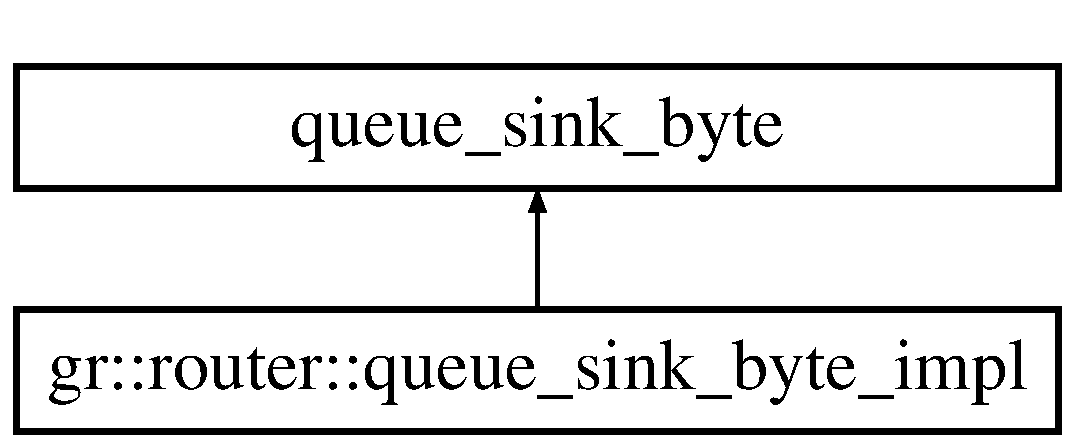
\includegraphics[height=2.000000cm]{classgr_1_1router_1_1queue__sink__byte__impl}
\end{center}
\end{figure}
\subsection*{Public Member Functions}
\begin{DoxyCompactItemize}
\item 
\hyperlink{classgr_1_1router_1_1queue__sink__byte__impl_a0ccee4dde1117105900ac5db604f98a6}{queue\+\_\+sink\+\_\+byte\+\_\+impl} (int item\+\_\+size, boost\+::lockfree\+::queue$<$ std\+::vector$<$ char $>$ $\ast$, boost\+::lockfree\+::fixed\+\_\+sized$<$ true $>$ $>$ \&shared\+\_\+queue, bool preserve\+\_\+index)
\item 
\hyperlink{classgr_1_1router_1_1queue__sink__byte__impl_a77245d6d769eddd788bcc7bc39be18e5}{$\sim$queue\+\_\+sink\+\_\+byte\+\_\+impl} ()
\item 
int \hyperlink{classgr_1_1router_1_1queue__sink__byte__impl_ac740a4bbd4bd2f5dabf1a33e28c9be92}{work} (int noutput\+\_\+items, gr\+\_\+vector\+\_\+const\+\_\+void\+\_\+star \&input\+\_\+items, gr\+\_\+vector\+\_\+void\+\_\+star \&output\+\_\+items)
\end{DoxyCompactItemize}


\subsection{Constructor \& Destructor Documentation}
\hypertarget{classgr_1_1router_1_1queue__sink__byte__impl_a0ccee4dde1117105900ac5db604f98a6}{\index{gr\+::router\+::queue\+\_\+sink\+\_\+byte\+\_\+impl@{gr\+::router\+::queue\+\_\+sink\+\_\+byte\+\_\+impl}!queue\+\_\+sink\+\_\+byte\+\_\+impl@{queue\+\_\+sink\+\_\+byte\+\_\+impl}}
\index{queue\+\_\+sink\+\_\+byte\+\_\+impl@{queue\+\_\+sink\+\_\+byte\+\_\+impl}!gr\+::router\+::queue\+\_\+sink\+\_\+byte\+\_\+impl@{gr\+::router\+::queue\+\_\+sink\+\_\+byte\+\_\+impl}}
\subsubsection[{queue\+\_\+sink\+\_\+byte\+\_\+impl}]{\setlength{\rightskip}{0pt plus 5cm}gr\+::router\+::queue\+\_\+sink\+\_\+byte\+\_\+impl\+::queue\+\_\+sink\+\_\+byte\+\_\+impl (
\begin{DoxyParamCaption}
\item[{int}]{size, }
\item[{boost\+::lockfree\+::queue$<$ std\+::vector$<$ char $>$ $\ast$, boost\+::lockfree\+::fixed\+\_\+sized$<$ true $>$ $>$ \&}]{shared\+\_\+queue, }
\item[{bool}]{preserve\+\_\+index}
\end{DoxyParamCaption}
)}}\label{classgr_1_1router_1_1queue__sink__byte__impl_a0ccee4dde1117105900ac5db604f98a6}
This is the public constructor for the queue\+\_\+sink\+\_\+byte block.


\begin{DoxyParams}{Parameters}
{\em size} & The size (in bytes) of the data being measured \\
\hline
{\em \&shared\+\_\+queue} & A reference to the shared queue where segments would be pushed. \\
\hline
{\em preserve\+\_\+index} & True if index is to be reconstructed from stream tags; generate new index from 0 otherwise. \\
\hline
\end{DoxyParams}
\hypertarget{classgr_1_1router_1_1queue__sink__byte__impl_a77245d6d769eddd788bcc7bc39be18e5}{\index{gr\+::router\+::queue\+\_\+sink\+\_\+byte\+\_\+impl@{gr\+::router\+::queue\+\_\+sink\+\_\+byte\+\_\+impl}!````~queue\+\_\+sink\+\_\+byte\+\_\+impl@{$\sim$queue\+\_\+sink\+\_\+byte\+\_\+impl}}
\index{````~queue\+\_\+sink\+\_\+byte\+\_\+impl@{$\sim$queue\+\_\+sink\+\_\+byte\+\_\+impl}!gr\+::router\+::queue\+\_\+sink\+\_\+byte\+\_\+impl@{gr\+::router\+::queue\+\_\+sink\+\_\+byte\+\_\+impl}}
\subsubsection[{$\sim$queue\+\_\+sink\+\_\+byte\+\_\+impl}]{\setlength{\rightskip}{0pt plus 5cm}gr\+::router\+::queue\+\_\+sink\+\_\+byte\+\_\+impl\+::$\sim$queue\+\_\+sink\+\_\+byte\+\_\+impl (
\begin{DoxyParamCaption}
{}
\end{DoxyParamCaption}
)}}\label{classgr_1_1router_1_1queue__sink__byte__impl_a77245d6d769eddd788bcc7bc39be18e5}
This is the destructor. 

\subsection{Member Function Documentation}
\hypertarget{classgr_1_1router_1_1queue__sink__byte__impl_ac740a4bbd4bd2f5dabf1a33e28c9be92}{\index{gr\+::router\+::queue\+\_\+sink\+\_\+byte\+\_\+impl@{gr\+::router\+::queue\+\_\+sink\+\_\+byte\+\_\+impl}!work@{work}}
\index{work@{work}!gr\+::router\+::queue\+\_\+sink\+\_\+byte\+\_\+impl@{gr\+::router\+::queue\+\_\+sink\+\_\+byte\+\_\+impl}}
\subsubsection[{work}]{\setlength{\rightskip}{0pt plus 5cm}int gr\+::router\+::queue\+\_\+sink\+\_\+byte\+\_\+impl\+::work (
\begin{DoxyParamCaption}
\item[{int}]{noutput\+\_\+items, }
\item[{gr\+\_\+vector\+\_\+const\+\_\+void\+\_\+star \&}]{input\+\_\+items, }
\item[{gr\+\_\+vector\+\_\+void\+\_\+star \&}]{output\+\_\+items}
\end{DoxyParamCaption}
)}}\label{classgr_1_1router_1_1queue__sink__byte__impl_ac740a4bbd4bd2f5dabf1a33e28c9be92}
This is the \hyperlink{classgr_1_1router_1_1queue__sink__byte__impl_ac740a4bbd4bd2f5dabf1a33e28c9be92}{work()} function of the queue sink byte block. 

The documentation for this class was generated from the following files\+:\begin{DoxyCompactItemize}
\item 
lib/queue\+\_\+sink\+\_\+byte\+\_\+impl.\+h\item 
lib/queue\+\_\+sink\+\_\+byte\+\_\+impl.\+cc\end{DoxyCompactItemize}

\hypertarget{classgr_1_1router_1_1queue__sink__impl}{\section{gr\+:\+:router\+:\+:queue\+\_\+sink\+\_\+impl Class Reference}
\label{classgr_1_1router_1_1queue__sink__impl}\index{gr\+::router\+::queue\+\_\+sink\+\_\+impl@{gr\+::router\+::queue\+\_\+sink\+\_\+impl}}
}
Inheritance diagram for gr\+:\+:router\+:\+:queue\+\_\+sink\+\_\+impl\+:\begin{figure}[H]
\begin{center}
\leavevmode
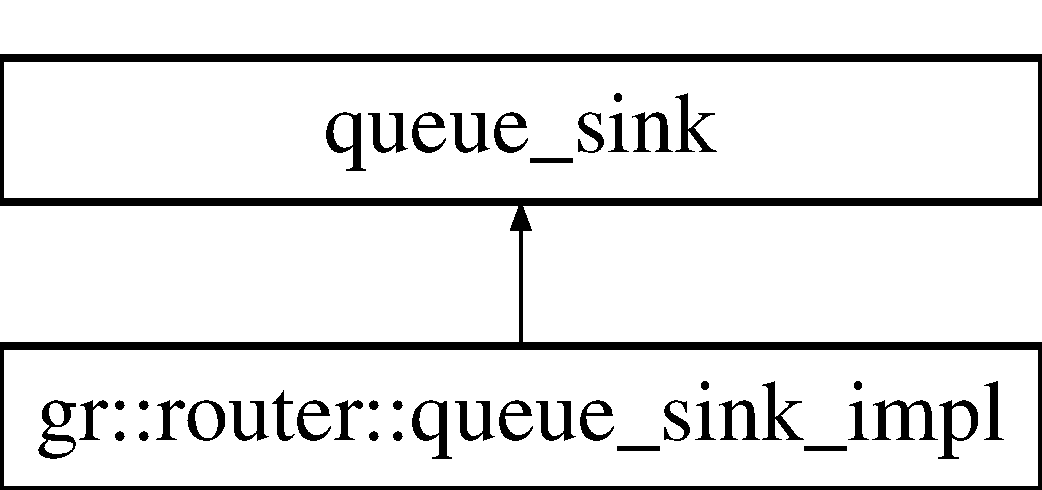
\includegraphics[height=2.000000cm]{classgr_1_1router_1_1queue__sink__impl}
\end{center}
\end{figure}
\subsection*{Public Member Functions}
\begin{DoxyCompactItemize}
\item 
\hyperlink{classgr_1_1router_1_1queue__sink__impl_aacd0fcad3ffba928c2782cc385c444d3}{queue\+\_\+sink\+\_\+impl} (int item\+\_\+size, boost\+::lockfree\+::queue$<$ std\+::vector$<$ float $>$ $\ast$, boost\+::lockfree\+::fixed\+\_\+sized$<$ true $>$ $>$ \&shared\+\_\+queue, bool preserve\+\_\+index)
\item 
\hyperlink{classgr_1_1router_1_1queue__sink__impl_ac503d2c10e679dd10c6ab4a6762dd22f}{$\sim$queue\+\_\+sink\+\_\+impl} ()
\item 
int \hyperlink{classgr_1_1router_1_1queue__sink__impl_a5762ae13eb5b07e1925e2e7266a33436}{work} (int noutput\+\_\+items, gr\+\_\+vector\+\_\+const\+\_\+void\+\_\+star \&input\+\_\+items, gr\+\_\+vector\+\_\+void\+\_\+star \&output\+\_\+items)
\end{DoxyCompactItemize}


\subsection{Constructor \& Destructor Documentation}
\hypertarget{classgr_1_1router_1_1queue__sink__impl_aacd0fcad3ffba928c2782cc385c444d3}{\index{gr\+::router\+::queue\+\_\+sink\+\_\+impl@{gr\+::router\+::queue\+\_\+sink\+\_\+impl}!queue\+\_\+sink\+\_\+impl@{queue\+\_\+sink\+\_\+impl}}
\index{queue\+\_\+sink\+\_\+impl@{queue\+\_\+sink\+\_\+impl}!gr\+::router\+::queue\+\_\+sink\+\_\+impl@{gr\+::router\+::queue\+\_\+sink\+\_\+impl}}
\subsubsection[{queue\+\_\+sink\+\_\+impl}]{\setlength{\rightskip}{0pt plus 5cm}gr\+::router\+::queue\+\_\+sink\+\_\+impl\+::queue\+\_\+sink\+\_\+impl (
\begin{DoxyParamCaption}
\item[{int}]{size, }
\item[{boost\+::lockfree\+::queue$<$ std\+::vector$<$ float $>$ $\ast$, boost\+::lockfree\+::fixed\+\_\+sized$<$ true $>$ $>$ \&}]{shared\+\_\+queue, }
\item[{bool}]{preserve\+\_\+index}
\end{DoxyParamCaption}
)}}\label{classgr_1_1router_1_1queue__sink__impl_aacd0fcad3ffba928c2782cc385c444d3}
This is the private constructor of the queue sick block.


\begin{DoxyParams}{Parameters}
{\em size} & The size (in bytes) of data units. \\
\hline
{\em \&shared\+\_\+queue} & A pointer to the fixed-\/sized lockfree queue in which the segments will be pushed. \\
\hline
{\em preserve\+\_\+index} & True if there is an index preserved in the stream tags, and if it is to be preserved in the resulting segments. Else, False. \\
\hline
\end{DoxyParams}
\hypertarget{classgr_1_1router_1_1queue__sink__impl_ac503d2c10e679dd10c6ab4a6762dd22f}{\index{gr\+::router\+::queue\+\_\+sink\+\_\+impl@{gr\+::router\+::queue\+\_\+sink\+\_\+impl}!````~queue\+\_\+sink\+\_\+impl@{$\sim$queue\+\_\+sink\+\_\+impl}}
\index{````~queue\+\_\+sink\+\_\+impl@{$\sim$queue\+\_\+sink\+\_\+impl}!gr\+::router\+::queue\+\_\+sink\+\_\+impl@{gr\+::router\+::queue\+\_\+sink\+\_\+impl}}
\subsubsection[{$\sim$queue\+\_\+sink\+\_\+impl}]{\setlength{\rightskip}{0pt plus 5cm}gr\+::router\+::queue\+\_\+sink\+\_\+impl\+::$\sim$queue\+\_\+sink\+\_\+impl (
\begin{DoxyParamCaption}
{}
\end{DoxyParamCaption}
)}}\label{classgr_1_1router_1_1queue__sink__impl_ac503d2c10e679dd10c6ab4a6762dd22f}
The destructor for the queue sink block. 

\subsection{Member Function Documentation}
\hypertarget{classgr_1_1router_1_1queue__sink__impl_a5762ae13eb5b07e1925e2e7266a33436}{\index{gr\+::router\+::queue\+\_\+sink\+\_\+impl@{gr\+::router\+::queue\+\_\+sink\+\_\+impl}!work@{work}}
\index{work@{work}!gr\+::router\+::queue\+\_\+sink\+\_\+impl@{gr\+::router\+::queue\+\_\+sink\+\_\+impl}}
\subsubsection[{work}]{\setlength{\rightskip}{0pt plus 5cm}int gr\+::router\+::queue\+\_\+sink\+\_\+impl\+::work (
\begin{DoxyParamCaption}
\item[{int}]{noutput\+\_\+items, }
\item[{gr\+\_\+vector\+\_\+const\+\_\+void\+\_\+star \&}]{input\+\_\+items, }
\item[{gr\+\_\+vector\+\_\+void\+\_\+star \&}]{output\+\_\+items}
\end{DoxyParamCaption}
)}}\label{classgr_1_1router_1_1queue__sink__impl_a5762ae13eb5b07e1925e2e7266a33436}
This is the \hyperlink{classgr_1_1router_1_1queue__sink__impl_a5762ae13eb5b07e1925e2e7266a33436}{work()} function. It segments the stream, and pushes the resulting segments into the lockfree queue.


\begin{DoxyParams}{Parameters}
{\em noutput\+\_\+items} & The number of data samples \\
\hline
{\em \&input\+\_\+items} & Pointer to input vector \\
\hline
{\em \&output\+\_\+items} & Pointer to output vector \\
\hline
\end{DoxyParams}


The documentation for this class was generated from the following files\+:\begin{DoxyCompactItemize}
\item 
lib/queue\+\_\+sink\+\_\+impl.\+h\item 
lib/queue\+\_\+sink\+\_\+impl.\+cc\end{DoxyCompactItemize}

\hypertarget{classgr_1_1router_1_1queue__source__byte__impl}{\section{gr\+:\+:router\+:\+:queue\+\_\+source\+\_\+byte\+\_\+impl Class Reference}
\label{classgr_1_1router_1_1queue__source__byte__impl}\index{gr\+::router\+::queue\+\_\+source\+\_\+byte\+\_\+impl@{gr\+::router\+::queue\+\_\+source\+\_\+byte\+\_\+impl}}
}
Inheritance diagram for gr\+:\+:router\+:\+:queue\+\_\+source\+\_\+byte\+\_\+impl\+:\begin{figure}[H]
\begin{center}
\leavevmode
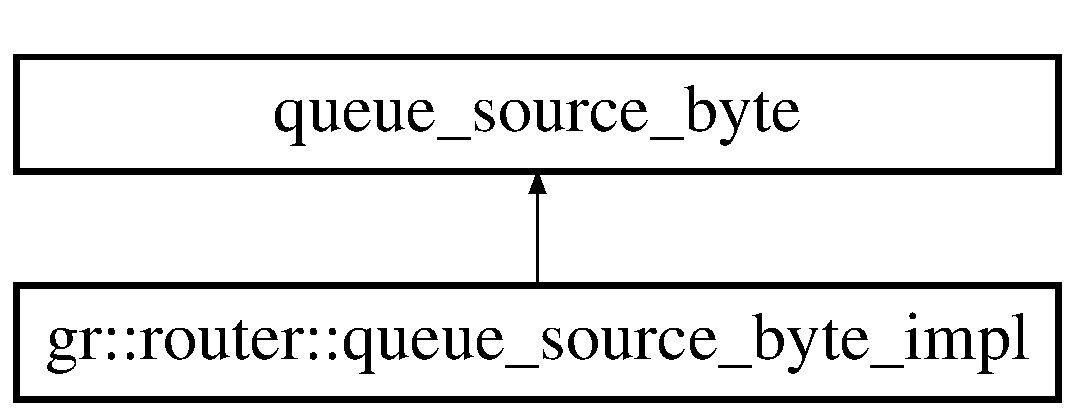
\includegraphics[height=2.000000cm]{classgr_1_1router_1_1queue__source__byte__impl}
\end{center}
\end{figure}
\subsection*{Public Member Functions}
\begin{DoxyCompactItemize}
\item 
\hyperlink{classgr_1_1router_1_1queue__source__byte__impl_af26965726f7f3c102c91e3cd78809070}{queue\+\_\+source\+\_\+byte\+\_\+impl} (int size, boost\+::lockfree\+::queue$<$ std\+::vector$<$ char $>$ $\ast$, boost\+::lockfree\+::fixed\+\_\+sized$<$ true $>$ $>$ \&shared\+\_\+queue, bool preserve\+\_\+index, bool order)
\item 
\hyperlink{classgr_1_1router_1_1queue__source__byte__impl_aa657da4357a0b8642ac71b07015934f3}{$\sim$queue\+\_\+source\+\_\+byte\+\_\+impl} ()
\item 
int \hyperlink{classgr_1_1router_1_1queue__source__byte__impl_acb768ac0c1e6e26a12e6cc31379ed415}{work} (int noutput\+\_\+items, gr\+\_\+vector\+\_\+const\+\_\+void\+\_\+star \&input\+\_\+items, gr\+\_\+vector\+\_\+void\+\_\+star \&output\+\_\+items)
\end{DoxyCompactItemize}


\subsection{Constructor \& Destructor Documentation}
\hypertarget{classgr_1_1router_1_1queue__source__byte__impl_af26965726f7f3c102c91e3cd78809070}{\index{gr\+::router\+::queue\+\_\+source\+\_\+byte\+\_\+impl@{gr\+::router\+::queue\+\_\+source\+\_\+byte\+\_\+impl}!queue\+\_\+source\+\_\+byte\+\_\+impl@{queue\+\_\+source\+\_\+byte\+\_\+impl}}
\index{queue\+\_\+source\+\_\+byte\+\_\+impl@{queue\+\_\+source\+\_\+byte\+\_\+impl}!gr\+::router\+::queue\+\_\+source\+\_\+byte\+\_\+impl@{gr\+::router\+::queue\+\_\+source\+\_\+byte\+\_\+impl}}
\subsubsection[{queue\+\_\+source\+\_\+byte\+\_\+impl}]{\setlength{\rightskip}{0pt plus 5cm}gr\+::router\+::queue\+\_\+source\+\_\+byte\+\_\+impl\+::queue\+\_\+source\+\_\+byte\+\_\+impl (
\begin{DoxyParamCaption}
\item[{int}]{size, }
\item[{boost\+::lockfree\+::queue$<$ std\+::vector$<$ char $>$ $\ast$, boost\+::lockfree\+::fixed\+\_\+sized$<$ true $>$ $>$ \&}]{shared\+\_\+queue, }
\item[{bool}]{preserve\+\_\+index, }
\item[{bool}]{order\+\_\+data}
\end{DoxyParamCaption}
)}}\label{classgr_1_1router_1_1queue__source__byte__impl_af26965726f7f3c102c91e3cd78809070}
The private constructor for the Queue Source.


\begin{DoxyParams}{Parameters}
{\em size} & The size of the samples in the stream in bytes. \\
\hline
{\em \&shared\+\_\+queue} & Reference to queue where segments will be popped from \\
\hline
{\em preserve\+\_\+index} & If the index of the segments is to be preserved in the resulting stream, True; else, False \\
\hline
{\em order\+\_\+data} & Require that all data parsed from queue segments be in the correct order before streaming. \\
\hline
\end{DoxyParams}
\hypertarget{classgr_1_1router_1_1queue__source__byte__impl_aa657da4357a0b8642ac71b07015934f3}{\index{gr\+::router\+::queue\+\_\+source\+\_\+byte\+\_\+impl@{gr\+::router\+::queue\+\_\+source\+\_\+byte\+\_\+impl}!````~queue\+\_\+source\+\_\+byte\+\_\+impl@{$\sim$queue\+\_\+source\+\_\+byte\+\_\+impl}}
\index{````~queue\+\_\+source\+\_\+byte\+\_\+impl@{$\sim$queue\+\_\+source\+\_\+byte\+\_\+impl}!gr\+::router\+::queue\+\_\+source\+\_\+byte\+\_\+impl@{gr\+::router\+::queue\+\_\+source\+\_\+byte\+\_\+impl}}
\subsubsection[{$\sim$queue\+\_\+source\+\_\+byte\+\_\+impl}]{\setlength{\rightskip}{0pt plus 5cm}gr\+::router\+::queue\+\_\+source\+\_\+byte\+\_\+impl\+::$\sim$queue\+\_\+source\+\_\+byte\+\_\+impl (
\begin{DoxyParamCaption}
{}
\end{DoxyParamCaption}
)}}\label{classgr_1_1router_1_1queue__source__byte__impl_aa657da4357a0b8642ac71b07015934f3}
The destructor. 

\subsection{Member Function Documentation}
\hypertarget{classgr_1_1router_1_1queue__source__byte__impl_acb768ac0c1e6e26a12e6cc31379ed415}{\index{gr\+::router\+::queue\+\_\+source\+\_\+byte\+\_\+impl@{gr\+::router\+::queue\+\_\+source\+\_\+byte\+\_\+impl}!work@{work}}
\index{work@{work}!gr\+::router\+::queue\+\_\+source\+\_\+byte\+\_\+impl@{gr\+::router\+::queue\+\_\+source\+\_\+byte\+\_\+impl}}
\subsubsection[{work}]{\setlength{\rightskip}{0pt plus 5cm}int gr\+::router\+::queue\+\_\+source\+\_\+byte\+\_\+impl\+::work (
\begin{DoxyParamCaption}
\item[{int}]{noutput\+\_\+items, }
\item[{gr\+\_\+vector\+\_\+const\+\_\+void\+\_\+star \&}]{input\+\_\+items, }
\item[{gr\+\_\+vector\+\_\+void\+\_\+star \&}]{output\+\_\+items}
\end{DoxyParamCaption}
)}}\label{classgr_1_1router_1_1queue__source__byte__impl_acb768ac0c1e6e26a12e6cc31379ed415}
The objective of the \hyperlink{classgr_1_1router_1_1queue__source__byte__impl_acb768ac0c1e6e26a12e6cc31379ed415}{work()} function is to grab windows from the shared\+\_\+queue and dump their contents into the out memory buffer.

If required, the windows are ordered prior to dumping their contents to maintain order across the flow graph.

Also, if the index of the window is to be maintained, the indexes are shared via stream tags. 

The documentation for this class was generated from the following files\+:\begin{DoxyCompactItemize}
\item 
lib/queue\+\_\+source\+\_\+byte\+\_\+impl.\+h\item 
lib/queue\+\_\+source\+\_\+byte\+\_\+impl.\+cc\end{DoxyCompactItemize}

\hypertarget{classgr_1_1router_1_1queue__source__impl}{\section{gr\+:\+:router\+:\+:queue\+\_\+source\+\_\+impl Class Reference}
\label{classgr_1_1router_1_1queue__source__impl}\index{gr\+::router\+::queue\+\_\+source\+\_\+impl@{gr\+::router\+::queue\+\_\+source\+\_\+impl}}
}
Inheritance diagram for gr\+:\+:router\+:\+:queue\+\_\+source\+\_\+impl\+:\begin{figure}[H]
\begin{center}
\leavevmode
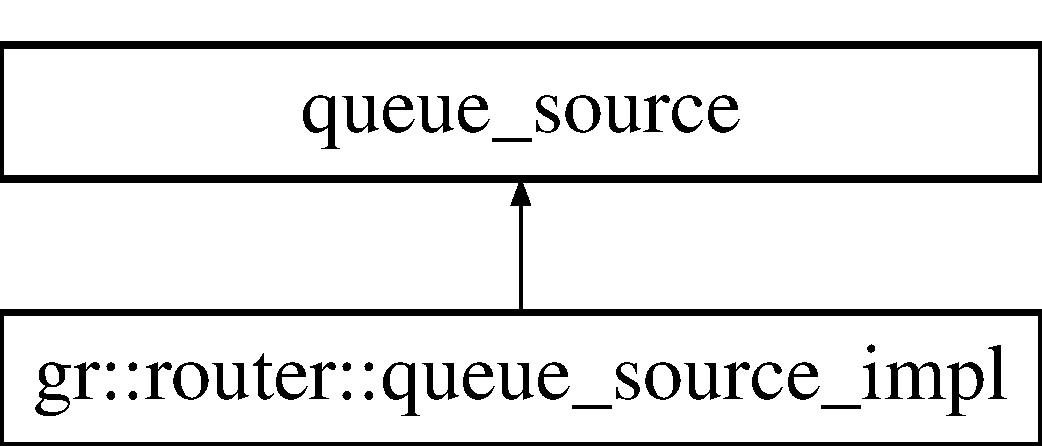
\includegraphics[height=2.000000cm]{classgr_1_1router_1_1queue__source__impl}
\end{center}
\end{figure}
\subsection*{Public Member Functions}
\begin{DoxyCompactItemize}
\item 
\hyperlink{classgr_1_1router_1_1queue__source__impl_a891c6664d0a1fda398cf66ea7e07fe1f}{queue\+\_\+source\+\_\+impl} (int size, boost\+::lockfree\+::queue$<$ std\+::vector$<$ float $>$ $\ast$, boost\+::lockfree\+::fixed\+\_\+sized$<$ true $>$ $>$ \&shared\+\_\+queue, bool preserve\+\_\+index, bool order)
\item 
\hyperlink{classgr_1_1router_1_1queue__source__impl_ac993c8ac719506456eb47ccf2016f5f0}{$\sim$queue\+\_\+source\+\_\+impl} ()
\item 
int \hyperlink{classgr_1_1router_1_1queue__source__impl_aecffa04879229acce72eb52da24dbfba}{work} (int noutput\+\_\+items, gr\+\_\+vector\+\_\+const\+\_\+void\+\_\+star \&input\+\_\+items, gr\+\_\+vector\+\_\+void\+\_\+star \&output\+\_\+items)
\end{DoxyCompactItemize}


\subsection{Constructor \& Destructor Documentation}
\hypertarget{classgr_1_1router_1_1queue__source__impl_a891c6664d0a1fda398cf66ea7e07fe1f}{\index{gr\+::router\+::queue\+\_\+source\+\_\+impl@{gr\+::router\+::queue\+\_\+source\+\_\+impl}!queue\+\_\+source\+\_\+impl@{queue\+\_\+source\+\_\+impl}}
\index{queue\+\_\+source\+\_\+impl@{queue\+\_\+source\+\_\+impl}!gr\+::router\+::queue\+\_\+source\+\_\+impl@{gr\+::router\+::queue\+\_\+source\+\_\+impl}}
\subsubsection[{queue\+\_\+source\+\_\+impl}]{\setlength{\rightskip}{0pt plus 5cm}gr\+::router\+::queue\+\_\+source\+\_\+impl\+::queue\+\_\+source\+\_\+impl (
\begin{DoxyParamCaption}
\item[{int}]{size, }
\item[{boost\+::lockfree\+::queue$<$ std\+::vector$<$ float $>$ $\ast$, boost\+::lockfree\+::fixed\+\_\+sized$<$ true $>$ $>$ \&}]{shared\+\_\+queue, }
\item[{bool}]{preserve\+\_\+index, }
\item[{bool}]{order\+\_\+data}
\end{DoxyParamCaption}
)}}\label{classgr_1_1router_1_1queue__source__impl_a891c6664d0a1fda398cf66ea7e07fe1f}
The private constructor for the Queue Source.


\begin{DoxyParams}{Parameters}
{\em size} & The size of the samples in the stream in bytes. \\
\hline
{\em \&shared\+\_\+queue} & Reference to queue where segments will be popped from \\
\hline
{\em preserve\+\_\+index} & If the index of the segments is to be preserved in the resulting stream, True; else, False \\
\hline
{\em order\+\_\+data} & Require that all data parsed from queue segments be in the correct order before streaming. \\
\hline
\end{DoxyParams}
\hypertarget{classgr_1_1router_1_1queue__source__impl_ac993c8ac719506456eb47ccf2016f5f0}{\index{gr\+::router\+::queue\+\_\+source\+\_\+impl@{gr\+::router\+::queue\+\_\+source\+\_\+impl}!````~queue\+\_\+source\+\_\+impl@{$\sim$queue\+\_\+source\+\_\+impl}}
\index{````~queue\+\_\+source\+\_\+impl@{$\sim$queue\+\_\+source\+\_\+impl}!gr\+::router\+::queue\+\_\+source\+\_\+impl@{gr\+::router\+::queue\+\_\+source\+\_\+impl}}
\subsubsection[{$\sim$queue\+\_\+source\+\_\+impl}]{\setlength{\rightskip}{0pt plus 5cm}gr\+::router\+::queue\+\_\+source\+\_\+impl\+::$\sim$queue\+\_\+source\+\_\+impl (
\begin{DoxyParamCaption}
{}
\end{DoxyParamCaption}
)}}\label{classgr_1_1router_1_1queue__source__impl_ac993c8ac719506456eb47ccf2016f5f0}
The destructor. 

\subsection{Member Function Documentation}
\hypertarget{classgr_1_1router_1_1queue__source__impl_aecffa04879229acce72eb52da24dbfba}{\index{gr\+::router\+::queue\+\_\+source\+\_\+impl@{gr\+::router\+::queue\+\_\+source\+\_\+impl}!work@{work}}
\index{work@{work}!gr\+::router\+::queue\+\_\+source\+\_\+impl@{gr\+::router\+::queue\+\_\+source\+\_\+impl}}
\subsubsection[{work}]{\setlength{\rightskip}{0pt plus 5cm}int gr\+::router\+::queue\+\_\+source\+\_\+impl\+::work (
\begin{DoxyParamCaption}
\item[{int}]{noutput\+\_\+items, }
\item[{gr\+\_\+vector\+\_\+const\+\_\+void\+\_\+star \&}]{input\+\_\+items, }
\item[{gr\+\_\+vector\+\_\+void\+\_\+star \&}]{output\+\_\+items}
\end{DoxyParamCaption}
)}}\label{classgr_1_1router_1_1queue__source__impl_aecffa04879229acce72eb52da24dbfba}
The objective of the \hyperlink{classgr_1_1router_1_1queue__source__impl_aecffa04879229acce72eb52da24dbfba}{work()} function is to grab windows from the shared\+\_\+queue and dump their contents into the out memory buffer.

If required, the windows are ordered prior to dumping their contents to maintain order across the flow graph.

Also, if the index of the window is to be maintained, the indexes are shared via stream tags. 

The documentation for this class was generated from the following files\+:\begin{DoxyCompactItemize}
\item 
lib/queue\+\_\+source\+\_\+impl.\+h\item 
lib/queue\+\_\+source\+\_\+impl.\+cc\end{DoxyCompactItemize}

\hypertarget{classgr_1_1router_1_1root__impl}{\section{gr\+:\+:router\+:\+:root\+\_\+impl Class Reference}
\label{classgr_1_1router_1_1root__impl}\index{gr\+::router\+::root\+\_\+impl@{gr\+::router\+::root\+\_\+impl}}
}
Inheritance diagram for gr\+:\+:router\+:\+:root\+\_\+impl\+:\begin{figure}[H]
\begin{center}
\leavevmode
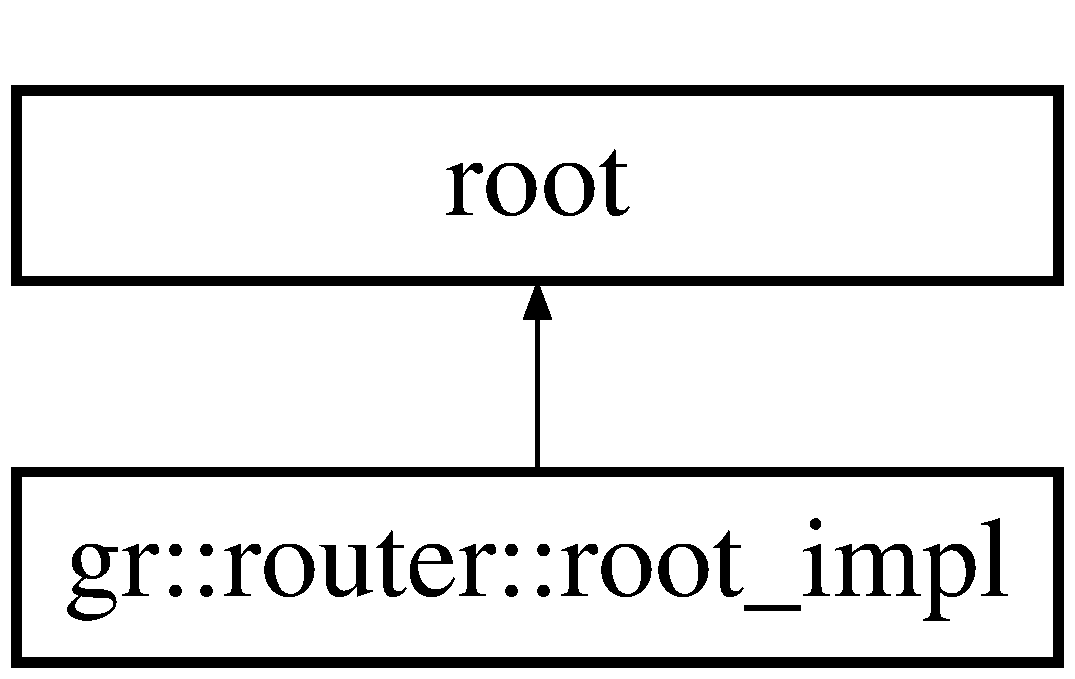
\includegraphics[height=2.000000cm]{classgr_1_1router_1_1root__impl}
\end{center}
\end{figure}
\subsection*{Public Member Functions}
\begin{DoxyCompactItemize}
\item 
\hyperlink{classgr_1_1router_1_1root__impl_ac848c67a6f8ca398d7ff7311ab4bb91d}{root\+\_\+impl} (int number\+\_\+of\+\_\+children, boost\+::lockfree\+::queue$<$ std\+::vector$<$ float $>$ $\ast$, boost\+::lockfree\+::fixed\+\_\+sized$<$ true $>$ $>$ \&in\+\_\+queue, boost\+::lockfree\+::queue$<$ std\+::vector$<$ char $>$ $\ast$, boost\+::lockfree\+::fixed\+\_\+sized$<$ true $>$ $>$ \&out\+\_\+queue, double throughput)
\item 
\hyperlink{classgr_1_1router_1_1root__impl_aba5b7eb8c530a435c1c2590cdd614ebc}{$\sim$root\+\_\+impl} ()
\item 
int \hyperlink{classgr_1_1router_1_1root__impl_ad2ac4750d299fecd92dd270f082ea189}{work} (int noutput\+\_\+items, gr\+\_\+vector\+\_\+const\+\_\+void\+\_\+star \&input\+\_\+items, gr\+\_\+vector\+\_\+void\+\_\+star \&output\+\_\+items)
\end{DoxyCompactItemize}


\subsection{Constructor \& Destructor Documentation}
\hypertarget{classgr_1_1router_1_1root__impl_ac848c67a6f8ca398d7ff7311ab4bb91d}{\index{gr\+::router\+::root\+\_\+impl@{gr\+::router\+::root\+\_\+impl}!root\+\_\+impl@{root\+\_\+impl}}
\index{root\+\_\+impl@{root\+\_\+impl}!gr\+::router\+::root\+\_\+impl@{gr\+::router\+::root\+\_\+impl}}
\subsubsection[{root\+\_\+impl}]{\setlength{\rightskip}{0pt plus 5cm}gr\+::router\+::root\+\_\+impl\+::root\+\_\+impl (
\begin{DoxyParamCaption}
\item[{int}]{numberofchildren, }
\item[{boost\+::lockfree\+::queue$<$ std\+::vector$<$ float $>$ $\ast$, boost\+::lockfree\+::fixed\+\_\+sized$<$ true $>$ $>$ \&}]{input\+\_\+queue, }
\item[{boost\+::lockfree\+::queue$<$ std\+::vector$<$ char $>$ $\ast$, boost\+::lockfree\+::fixed\+\_\+sized$<$ true $>$ $>$ \&}]{output\+\_\+queue, }
\item[{double}]{throughput}
\end{DoxyParamCaption}
)}}\label{classgr_1_1router_1_1root__impl_ac848c67a6f8ca398d7ff7311ab4bb91d}
The private constructor for the Root router.


\begin{DoxyParams}{Parameters}
{\em number\+\_\+of\+\_\+children} & The number of children under this node. \\
\hline
{\em \&input\+\_\+queue} & Reference to input queue to push computable segments to. \\
\hline
{\em \&output\+\_\+queue} & Reference to output queue to pop result segments from. \\
\hline
{\em throughput} & The maximum rate at which segments are popped from the output queue \\
\hline
\end{DoxyParams}
\hypertarget{classgr_1_1router_1_1root__impl_aba5b7eb8c530a435c1c2590cdd614ebc}{\index{gr\+::router\+::root\+\_\+impl@{gr\+::router\+::root\+\_\+impl}!````~root\+\_\+impl@{$\sim$root\+\_\+impl}}
\index{````~root\+\_\+impl@{$\sim$root\+\_\+impl}!gr\+::router\+::root\+\_\+impl@{gr\+::router\+::root\+\_\+impl}}
\subsubsection[{$\sim$root\+\_\+impl}]{\setlength{\rightskip}{0pt plus 5cm}gr\+::router\+::root\+\_\+impl\+::$\sim$root\+\_\+impl (
\begin{DoxyParamCaption}
{}
\end{DoxyParamCaption}
)}}\label{classgr_1_1router_1_1root__impl_aba5b7eb8c530a435c1c2590cdd614ebc}
The destructor for the root router block. 

\subsection{Member Function Documentation}
\hypertarget{classgr_1_1router_1_1root__impl_ad2ac4750d299fecd92dd270f082ea189}{\index{gr\+::router\+::root\+\_\+impl@{gr\+::router\+::root\+\_\+impl}!work@{work}}
\index{work@{work}!gr\+::router\+::root\+\_\+impl@{gr\+::router\+::root\+\_\+impl}}
\subsubsection[{work}]{\setlength{\rightskip}{0pt plus 5cm}int gr\+::router\+::root\+\_\+impl\+::work (
\begin{DoxyParamCaption}
\item[{int}]{noutput\+\_\+items, }
\item[{gr\+\_\+vector\+\_\+const\+\_\+void\+\_\+star \&}]{input\+\_\+items, }
\item[{gr\+\_\+vector\+\_\+void\+\_\+star \&}]{output\+\_\+items}
\end{DoxyParamCaption}
)}}\label{classgr_1_1router_1_1root__impl_ad2ac4750d299fecd92dd270f082ea189}
Unused \hyperlink{classgr_1_1router_1_1root__impl_ad2ac4750d299fecd92dd270f082ea189}{work()} function; this block is independently threaded. 

The documentation for this class was generated from the following files\+:\begin{DoxyCompactItemize}
\item 
lib/root\+\_\+impl.\+h\item 
lib/root\+\_\+impl.\+cc\end{DoxyCompactItemize}

\hypertarget{classgr_1_1router_1_1throughput__impl}{\section{gr\+:\+:router\+:\+:throughput\+\_\+impl Class Reference}
\label{classgr_1_1router_1_1throughput__impl}\index{gr\+::router\+::throughput\+\_\+impl@{gr\+::router\+::throughput\+\_\+impl}}
}
Inheritance diagram for gr\+:\+:router\+:\+:throughput\+\_\+impl\+:\begin{figure}[H]
\begin{center}
\leavevmode
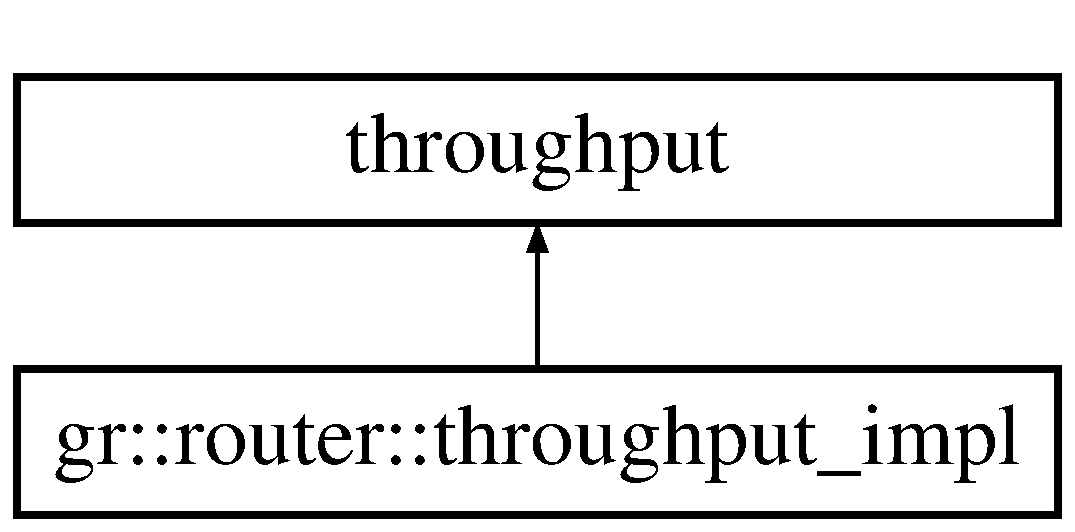
\includegraphics[height=2.000000cm]{classgr_1_1router_1_1throughput__impl}
\end{center}
\end{figure}
\subsection*{Public Member Functions}
\begin{DoxyCompactItemize}
\item 
\hyperlink{classgr_1_1router_1_1throughput__impl_a4c435290b81331a3d7079e718a3b0326}{throughput\+\_\+impl} (size\+\_\+t itemsize, int print\+\_\+counter, int index)
\item 
\hyperlink{classgr_1_1router_1_1throughput__impl_a8ef92f4e626f69b8c18cb93c26969fd3}{$\sim$throughput\+\_\+impl} ()
\item 
int \hyperlink{classgr_1_1router_1_1throughput__impl_aafd5b37bbffbdb5ae5248f85fab76050}{work} (int noutput\+\_\+items, gr\+\_\+vector\+\_\+const\+\_\+void\+\_\+star \&input\+\_\+items, gr\+\_\+vector\+\_\+void\+\_\+star \&output\+\_\+items)
\end{DoxyCompactItemize}


\subsection{Constructor \& Destructor Documentation}
\hypertarget{classgr_1_1router_1_1throughput__impl_a4c435290b81331a3d7079e718a3b0326}{\index{gr\+::router\+::throughput\+\_\+impl@{gr\+::router\+::throughput\+\_\+impl}!throughput\+\_\+impl@{throughput\+\_\+impl}}
\index{throughput\+\_\+impl@{throughput\+\_\+impl}!gr\+::router\+::throughput\+\_\+impl@{gr\+::router\+::throughput\+\_\+impl}}
\subsubsection[{throughput\+\_\+impl}]{\setlength{\rightskip}{0pt plus 5cm}gr\+::router\+::throughput\+\_\+impl\+::throughput\+\_\+impl (
\begin{DoxyParamCaption}
\item[{size\+\_\+t}]{itemsize, }
\item[{int}]{print\+\_\+counter, }
\item[{int}]{index}
\end{DoxyParamCaption}
)}}\label{classgr_1_1router_1_1throughput__impl_a4c435290b81331a3d7079e718a3b0326}
This is the private constructor for the throughput block.


\begin{DoxyParams}{Parameters}
{\em itemsize} & The size (in bytes) of the data being measured \\
\hline
{\em print\+\_\+counter} & The number of \hyperlink{classgr_1_1router_1_1throughput__impl_aafd5b37bbffbdb5ae5248f85fab76050}{work()} calls between prints of throughput value \\
\hline
{\em index} & How many tabs in front of the throughput value to space them \\
\hline
\end{DoxyParams}
\hypertarget{classgr_1_1router_1_1throughput__impl_a8ef92f4e626f69b8c18cb93c26969fd3}{\index{gr\+::router\+::throughput\+\_\+impl@{gr\+::router\+::throughput\+\_\+impl}!````~throughput\+\_\+impl@{$\sim$throughput\+\_\+impl}}
\index{````~throughput\+\_\+impl@{$\sim$throughput\+\_\+impl}!gr\+::router\+::throughput\+\_\+impl@{gr\+::router\+::throughput\+\_\+impl}}
\subsubsection[{$\sim$throughput\+\_\+impl}]{\setlength{\rightskip}{0pt plus 5cm}gr\+::router\+::throughput\+\_\+impl\+::$\sim$throughput\+\_\+impl (
\begin{DoxyParamCaption}
{}
\end{DoxyParamCaption}
)}}\label{classgr_1_1router_1_1throughput__impl_a8ef92f4e626f69b8c18cb93c26969fd3}
The destructor for the throughput block. 

\subsection{Member Function Documentation}
\hypertarget{classgr_1_1router_1_1throughput__impl_aafd5b37bbffbdb5ae5248f85fab76050}{\index{gr\+::router\+::throughput\+\_\+impl@{gr\+::router\+::throughput\+\_\+impl}!work@{work}}
\index{work@{work}!gr\+::router\+::throughput\+\_\+impl@{gr\+::router\+::throughput\+\_\+impl}}
\subsubsection[{work}]{\setlength{\rightskip}{0pt plus 5cm}int gr\+::router\+::throughput\+\_\+impl\+::work (
\begin{DoxyParamCaption}
\item[{int}]{noutput\+\_\+items, }
\item[{gr\+\_\+vector\+\_\+const\+\_\+void\+\_\+star \&}]{input\+\_\+items, }
\item[{gr\+\_\+vector\+\_\+void\+\_\+star \&}]{output\+\_\+items}
\end{DoxyParamCaption}
)}}\label{classgr_1_1router_1_1throughput__impl_aafd5b37bbffbdb5ae5248f85fab76050}
This is the \hyperlink{classgr_1_1router_1_1throughput__impl_aafd5b37bbffbdb5ae5248f85fab76050}{work()} function. It prints the average throughput to std\+::out every d\+\_\+print\+\_\+counter times \hyperlink{classgr_1_1router_1_1throughput__impl_aafd5b37bbffbdb5ae5248f85fab76050}{work()} is called.

This block is transparent and the data on the input is copied to the output.


\begin{DoxyParams}{Parameters}
{\em noutput\+\_\+items} & The number of data samples \\
\hline
{\em \&input\+\_\+items} & Pointer to input vector \\
\hline
{\em \&output\+\_\+items} & Pointer to output vector \\
\hline
\end{DoxyParams}


The documentation for this class was generated from the following files\+:\begin{DoxyCompactItemize}
\item 
lib/throughput\+\_\+impl.\+h\item 
lib/throughput\+\_\+impl.\+cc\end{DoxyCompactItemize}

\hypertarget{classgr_1_1router_1_1throughput__sink__impl}{\section{gr\+:\+:router\+:\+:throughput\+\_\+sink\+\_\+impl Class Reference}
\label{classgr_1_1router_1_1throughput__sink__impl}\index{gr\+::router\+::throughput\+\_\+sink\+\_\+impl@{gr\+::router\+::throughput\+\_\+sink\+\_\+impl}}
}
Inheritance diagram for gr\+:\+:router\+:\+:throughput\+\_\+sink\+\_\+impl\+:\begin{figure}[H]
\begin{center}
\leavevmode
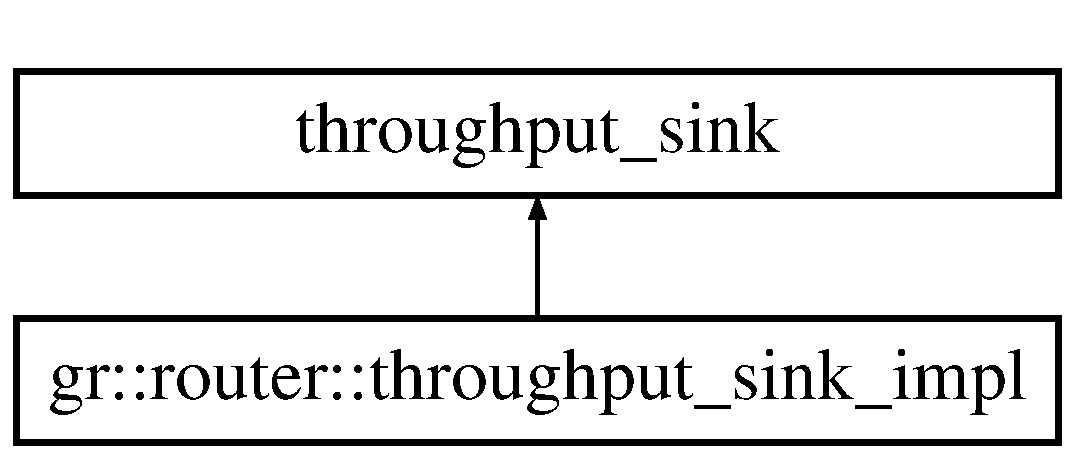
\includegraphics[height=2.000000cm]{classgr_1_1router_1_1throughput__sink__impl}
\end{center}
\end{figure}
\subsection*{Public Member Functions}
\begin{DoxyCompactItemize}
\item 
\hyperlink{classgr_1_1router_1_1throughput__sink__impl_a8e9ff88368998958c08b3333ffd37f22}{throughput\+\_\+sink\+\_\+impl} (size\+\_\+t itemsize, int print\+\_\+counter, int index)
\item 
\hyperlink{classgr_1_1router_1_1throughput__sink__impl_a017767ebc428bfece5be62f74b6ca203}{$\sim$throughput\+\_\+sink\+\_\+impl} ()
\item 
int \hyperlink{classgr_1_1router_1_1throughput__sink__impl_aec208c69fd29cd4ab20334bf373bf7e6}{work} (int noutput\+\_\+items, gr\+\_\+vector\+\_\+const\+\_\+void\+\_\+star \&input\+\_\+items, gr\+\_\+vector\+\_\+void\+\_\+star \&output\+\_\+items)
\end{DoxyCompactItemize}


\subsection{Constructor \& Destructor Documentation}
\hypertarget{classgr_1_1router_1_1throughput__sink__impl_a8e9ff88368998958c08b3333ffd37f22}{\index{gr\+::router\+::throughput\+\_\+sink\+\_\+impl@{gr\+::router\+::throughput\+\_\+sink\+\_\+impl}!throughput\+\_\+sink\+\_\+impl@{throughput\+\_\+sink\+\_\+impl}}
\index{throughput\+\_\+sink\+\_\+impl@{throughput\+\_\+sink\+\_\+impl}!gr\+::router\+::throughput\+\_\+sink\+\_\+impl@{gr\+::router\+::throughput\+\_\+sink\+\_\+impl}}
\subsubsection[{throughput\+\_\+sink\+\_\+impl}]{\setlength{\rightskip}{0pt plus 5cm}gr\+::router\+::throughput\+\_\+sink\+\_\+impl\+::throughput\+\_\+sink\+\_\+impl (
\begin{DoxyParamCaption}
\item[{size\+\_\+t}]{itemsize, }
\item[{int}]{print\+\_\+counter, }
\item[{int}]{index}
\end{DoxyParamCaption}
)}}\label{classgr_1_1router_1_1throughput__sink__impl_a8e9ff88368998958c08b3333ffd37f22}
This is the private constructor for the throughput block.


\begin{DoxyParams}{Parameters}
{\em itemsize} & The size (in bytes) of the data being measured \\
\hline
{\em print\+\_\+counter} & The number of \hyperlink{classgr_1_1router_1_1throughput__sink__impl_aec208c69fd29cd4ab20334bf373bf7e6}{work()} calls between prints of throughput value \\
\hline
{\em index} & How many tabs in front of the throughput value to space them \\
\hline
\end{DoxyParams}
\hypertarget{classgr_1_1router_1_1throughput__sink__impl_a017767ebc428bfece5be62f74b6ca203}{\index{gr\+::router\+::throughput\+\_\+sink\+\_\+impl@{gr\+::router\+::throughput\+\_\+sink\+\_\+impl}!````~throughput\+\_\+sink\+\_\+impl@{$\sim$throughput\+\_\+sink\+\_\+impl}}
\index{````~throughput\+\_\+sink\+\_\+impl@{$\sim$throughput\+\_\+sink\+\_\+impl}!gr\+::router\+::throughput\+\_\+sink\+\_\+impl@{gr\+::router\+::throughput\+\_\+sink\+\_\+impl}}
\subsubsection[{$\sim$throughput\+\_\+sink\+\_\+impl}]{\setlength{\rightskip}{0pt plus 5cm}gr\+::router\+::throughput\+\_\+sink\+\_\+impl\+::$\sim$throughput\+\_\+sink\+\_\+impl (
\begin{DoxyParamCaption}
{}
\end{DoxyParamCaption}
)}}\label{classgr_1_1router_1_1throughput__sink__impl_a017767ebc428bfece5be62f74b6ca203}
This is the destructor for the throughput sink block. 

\subsection{Member Function Documentation}
\hypertarget{classgr_1_1router_1_1throughput__sink__impl_aec208c69fd29cd4ab20334bf373bf7e6}{\index{gr\+::router\+::throughput\+\_\+sink\+\_\+impl@{gr\+::router\+::throughput\+\_\+sink\+\_\+impl}!work@{work}}
\index{work@{work}!gr\+::router\+::throughput\+\_\+sink\+\_\+impl@{gr\+::router\+::throughput\+\_\+sink\+\_\+impl}}
\subsubsection[{work}]{\setlength{\rightskip}{0pt plus 5cm}int gr\+::router\+::throughput\+\_\+sink\+\_\+impl\+::work (
\begin{DoxyParamCaption}
\item[{int}]{noutput\+\_\+items, }
\item[{gr\+\_\+vector\+\_\+const\+\_\+void\+\_\+star \&}]{input\+\_\+items, }
\item[{gr\+\_\+vector\+\_\+void\+\_\+star \&}]{output\+\_\+items}
\end{DoxyParamCaption}
)}}\label{classgr_1_1router_1_1throughput__sink__impl_aec208c69fd29cd4ab20334bf373bf7e6}
This is the \hyperlink{classgr_1_1router_1_1throughput__sink__impl_aec208c69fd29cd4ab20334bf373bf7e6}{work()} function of the throughput\+\_\+sink 

The documentation for this class was generated from the following files\+:\begin{DoxyCompactItemize}
\item 
lib/throughput\+\_\+sink\+\_\+impl.\+h\item 
lib/throughput\+\_\+sink\+\_\+impl.\+cc\end{DoxyCompactItemize}

%--- End generated contents ---

% Index
\newpage
\phantomsection
\addcontentsline{toc}{chapter}{Index}
\printindex

\end{document}
